\documentclass{standalone}
\usepackage{tikz}
\usepackage{tikz-cd}
\usepackage{tikz-3dplot}
\usepackage{pgfplots}
\usepackage{pgffor} % For \foreach loop
\pgfplotsset{compat=newest} % Adjust to your version of pgfplots
\def\Circlearrowleft{\ensuremath{%
		\rotatebox[origin=c]{180}{$\circlearrowleft$}}}
\def\Circlearrowright{\ensuremath{%
		\rotatebox[origin=c]{180}{$\circlearrowright$}}}
\def\CircleArrowleft{\ensuremath{%
		\reflectbox{\rotatebox[origin=c]{180}{$\circlearrowleft$}}}}
\def\CircleArrowright{\ensuremath{%
		\reflectbox{\rotatebox[origin=c]{180}{$\circlearrowright$}}}}
\usetikzlibrary{
	3d, % For 3D drawing
	angles,
	arrows,
	arrows.meta,
	backgrounds,
	bending,
	calc,
	decorations.pathmorphing,
	decorations.pathreplacing,
	decorations.markings,
	fit,
	matrix,
	patterns,
	patterns.meta,
	positioning,
	quotes,
	shadows,
	shapes,
	shapes.geometric
}
\newcommand{\thickprohibit}{%
	
\begin{tikzpicture}
		% Adjust 'thick' to 'very thick' or line width for thicker circle
		\draw[line width=1mm] (0,0) circle (1);
		% Adjust 'thick' to 'very thick' or line width for thicker line
		\draw[line width=1mm] (-0.707,-0.707) -- (0.707,0.707); 
	\end{tikzpicture}
}
% Define the command with parameters for size and line width
\def\mythickprohibit#1#2{%
	\begin{tikzpicture}
		\draw[line width=#2] (0,0) circle (#1); % Circle with variable size and line width
		\draw[line width=#2] (-0.707*#1,-0.707*#1) -- (0.707*#1,0.707*#1); % Diagonal line
	\end{tikzpicture}
}
\begin{document}
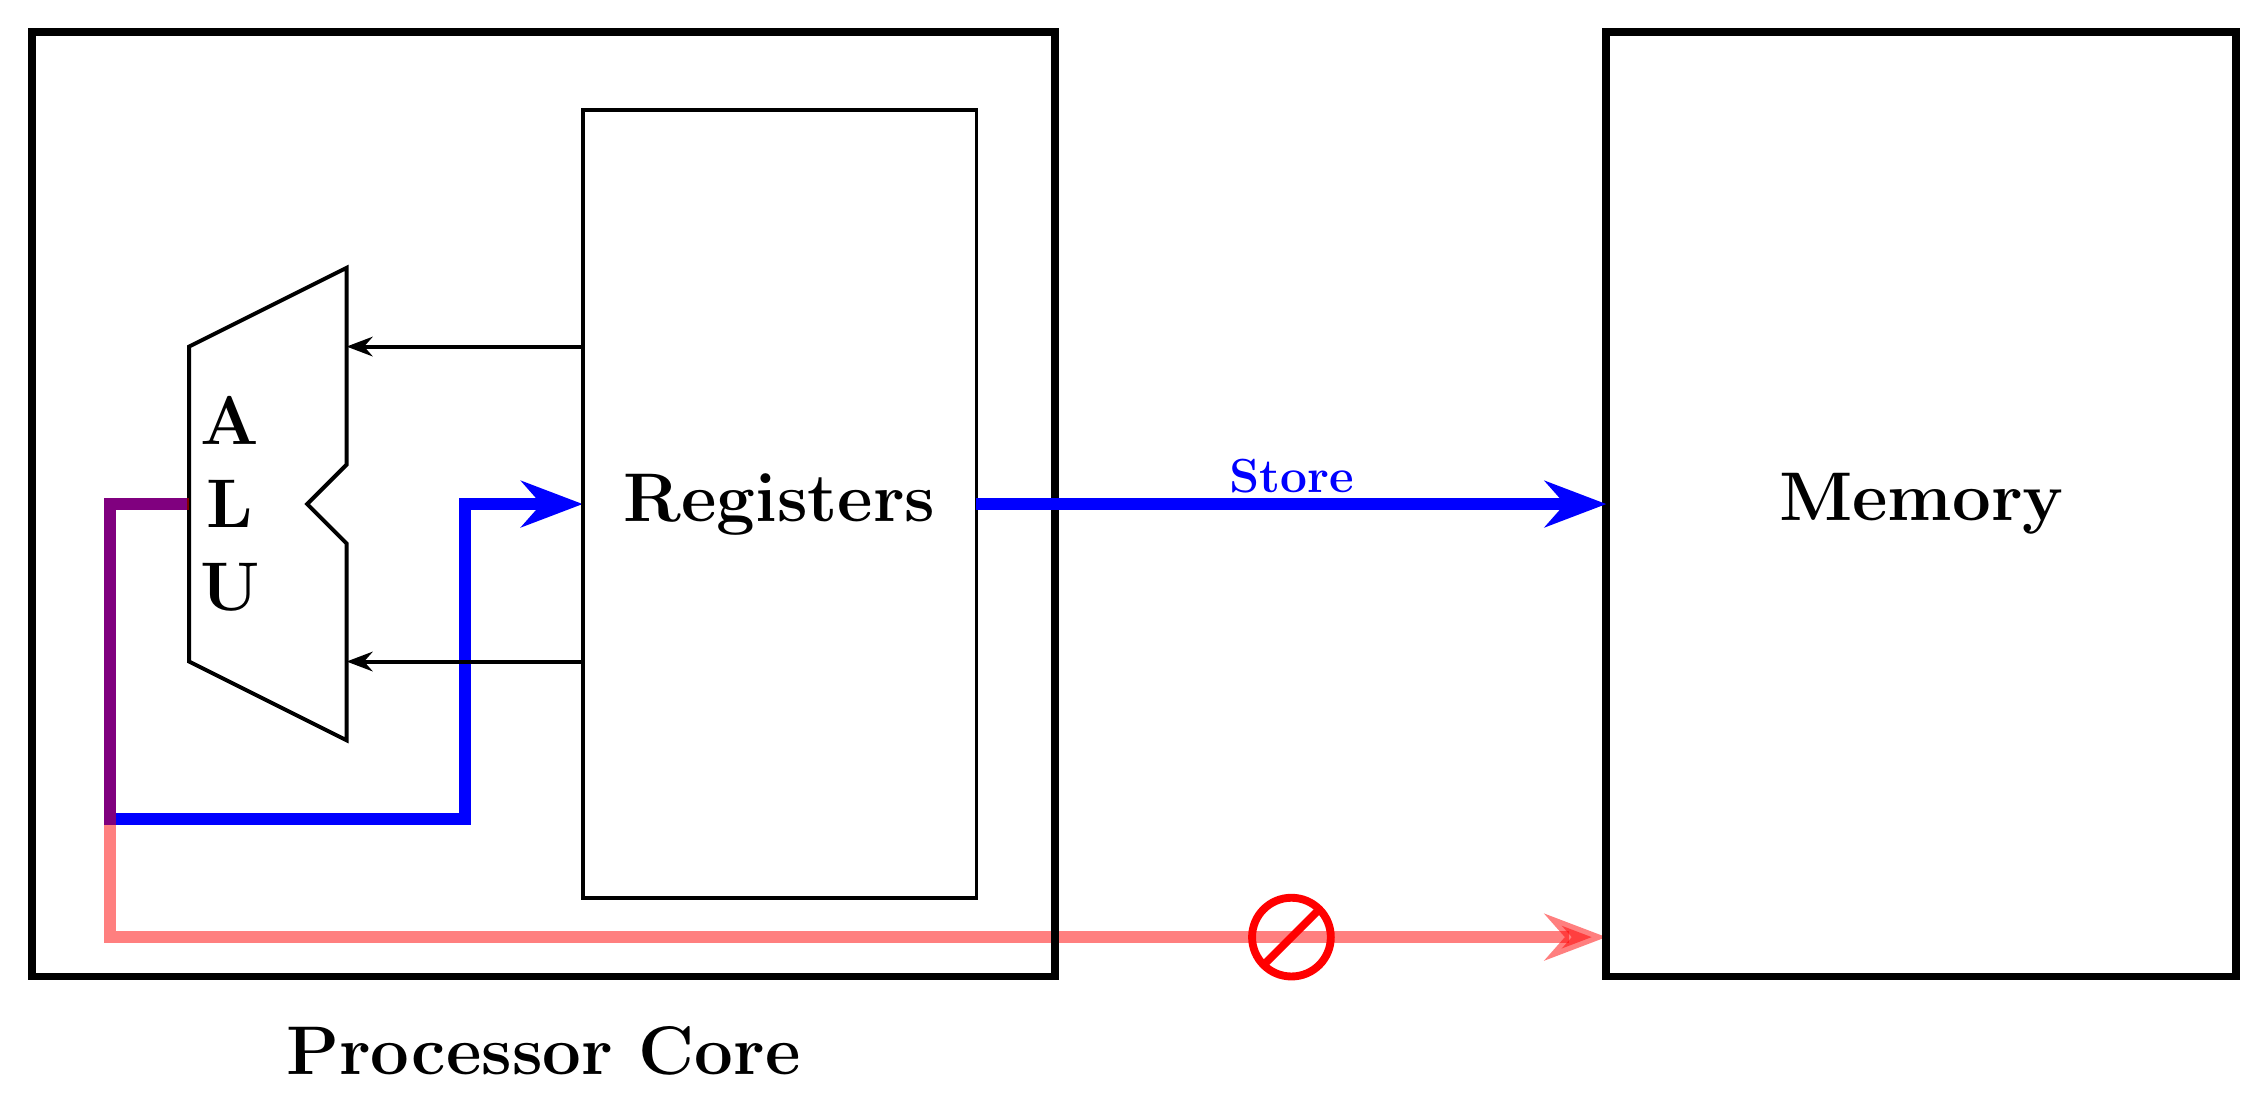
\begin{tikzpicture}[>=Stealth, line width=.5mm]
	\def \x{15}
	\def \y{10}
%	\draw[very thin,color=gray!15,step=.5] (-\x,-\y) grid (\x,\y);
%	
%	\foreach \i in {-\x,...,-2,-1,1,2,...,\x}
%	\draw[gray] (\i,.1)--(\i,-.1) node[below] {$\i$};%x-axis
%	\foreach \i in {-\y,-1,1,1,\y}
%	\draw[gray] (.1,\i)--(-.1,\i) node[left] {$\i$};%y-axis
	
	\begin{scope}[xshift=-2cm]
	% ALU Section (at x = -2)
	\draw[blue, ->, line width=1.5mm] (-10, 0) -- (-11, 0) -- (-11,-4) |- (-6.5,-4) -- (-6.5, 0) -- (-5,0);
	\draw[] (-10, -2) -- (-8, -3) -- (-8, -.5) -- (-8.5, 0) -- (-8, .5) -- (-8, 3) -- (-10, 2) -- cycle node[midway, right, align=center] {\Huge\bf A\\ \ \\ \Huge\bf L\\ \ \\ \Huge\bf U};
	\draw[red, ->, line width=1.5mm, opacity=.5] (-10, 0) -- (-11, 0) -- (-11,-5.5) |- (8,-5.5);
	\node[red] at (4,-5.5) {\mythickprohibit{.5}{1mm}};
	\draw[->] (-5, 2) to (-8, 2);
	\draw[->] (-5, -2) to (-8, -2);


	% Registers section (left side)
	\node[] at (-2.5, 0) {\Huge\bf Registers};
	\draw[] (-5, -5) rectangle (0, 5); % Outer box
	\draw[line width=1mm] (-12, -6) rectangle (1, 6);
	\node[below] at (-5.5, -6.5) {\Huge\bf Processor Core};
	\end{scope}
	
	% Memory section (right side)
	\begin{scope}[xshift=7cm]
	\draw[line width=1mm] (-1, -6) rectangle (7, 6);
	\node[] at (3, 0) {\Huge\bf Memory};
	
	\draw[blue, <-, line width=1.5mm] (-1,0) to (-9,0);
	\node[blue, above] at (-5,0) {\LARGE\bf Store};
	\end{scope}
\end{tikzpicture}
\end{document}
